\documentclass{article}
\usepackage[utf8]{inputenc}

\title{PRD Energy Reconstruction}
\author{Xianyi Zhang}
\date{December 2018}

\usepackage{natbib}
\usepackage{graphicx}

\begin{document}

\maketitle

\section{Energy Reconstruction}
% reconstruction mechanics - electronic signal to physics
The energy deposit in each segment was reconstructed with respect to the light collected with the PMTs on both ends.
The pulse integral of the PMT light collection was converted to the event energy by tracking the neutron-lithium capture energy distribution ($\sim$0.6~MeVee), which is well localized in PSD, energy and position parameter space.
To balance the data recording throughput with small energy deposition, the data acquisition was triggered upon $\sim$150~keV threshold in any segment. 
Once data acquisition was triggered, a zero-length encoding (ZLE) threshold allows any PMT signal exceeding $\sim$2~PE to be stored.

% reconstruction mechanics - reconstructed energy
Given the segmented nature of the PROSPECT AD, a incident particle can deposit energy in multiple segments before stopped.
An event's total reconstucted energy is the summed energy deposit in segments with 20~ns time interval.
Because of the light attenuation in LiLS, the $\sim$2~PE ZLE threshold could cause position dependent exclusion of low energy deposition and result in non-uniform reconstructed energy.
An 85~keV (TODO: update this value) analysis threshold was applied on energy deposit in each segment to unify the reconstructed energy.
Since variation of energy resolution among segments during the data acquisition was observed, a event-level smearing of energy resolution was applied, which was equivalent to 400 PE/MeV photostatistics or 5\% at 1 MeV.

% calibration used
The PROSPECT AD energy response was calibrated with detector center deployed radioactive sources and environmental radiations.
The energy response was simulated with PROSPECT's custom build Geant4 Monte Carlo simulation package (PG4).
A combined data-MC comparison of cosmogenic $^{12}$B $\beta$-decay, neutron-hydrogen capture $\gamma$-ray, and $\gamma$-ray from deployed radioactive sources, including $^{60}$Co, $^{137}$Cs and $^{22}$Na, were made to constrain the energy response model in PG4 simulation.

% energy response model
The nonlinearity of reconstructed energy were modeled with Birks' law quenching and Cherenkov radiation.
In the PG4 simulation, the energy nonlinearity was simulated by correction applied on energy deposition of each G4Step of particle, where the $E$ and $dE/dx$ was calculated.
The Birks' law quenching correction,
\begin{equation}
    \frac{dL}{dx} = \frac{\frac{dE}{dx}}{1+k_{B1}\frac{dE}{dx}+k_{B2}(\frac{dE}{dx})^2},
\end{equation}
was implemented, where $\frac{dL}{dx}$ is energy deposition per step, $k_{B1}$ and $k_{B2}$ are the first and second Birks' constants.
The Cherenkov radiation was simulated by assuming uniform amount of photon was generated in 200-700~nm wavelength band, and the number of photon per step per band is  
\begin{equation}
    \frac{d^2N}{dxd\lambda} = \frac{2\pi\alpha z^2}{\lambda}\left(1- \frac{1}{\beta^2n^2(\lambda)}\right),
\end{equation}
where $N$ is number of photon, $\alpha$ is fine-structure constant, $\beta$ is the speed of the particle, and $n$ is index of refraction.
The energy correction of Cherenkov radiation was the summed energy of Cherenkov photon multiplied with a simulated detection efficiency $k_{C}$, as
\begin{equation}
    E_{Ckov} = k_{C}\sum_{\lambda}N_\lambda E_\lambda.
\end{equation}

%combined fitting
To constrain the energy response model, the energy spectra of calibration data and MC were compared simultaneously with the summed $\chi^2$.
In addition, the segmentation of PROSPECT AD was non-negligible in energy reconstruction. 
The multi-segment-scattering of higher energy particles travel in the detector introduced complicated nonlinear effects of reconstructed energy that dependent on segment multiplicity.
Thus, the multiplicities of $\gamma$-ray events from $^{60}$Co, $^{137}$Cs and $^{22}$Na calibrations was also compared between data and MC, and the $\chi^2$ values were added in the summed $\chi^2$ of the spectral comparisons.
The $k_{B1}$, $k_{B2}$, $k_{C}$, and an absolute energy scale constant $\beta$ were allowed to float in the combined data-MC until the summed $\chi^2$ was minimized.
The absolute scale $\beta$ was used to cancel a possible systematic bias because the exact energy of neutron-lithium capture, which was used in pulse-energy conversion, was not accurately determined.
When the best fit energy response model between calibration data and corresponding data was found, all data was re-calibrated so $\beta$ could be fixed to 1. 
The reconstructed energy spectra and best fit MC spectra are shown in Figure \ref{fig:gammacalibration}.
The multiplicities of $\gamma$-ray calibrations and best fit MC are shown in Figure \ref{fig:multi}.

\begin{figure}[h!]
\centering
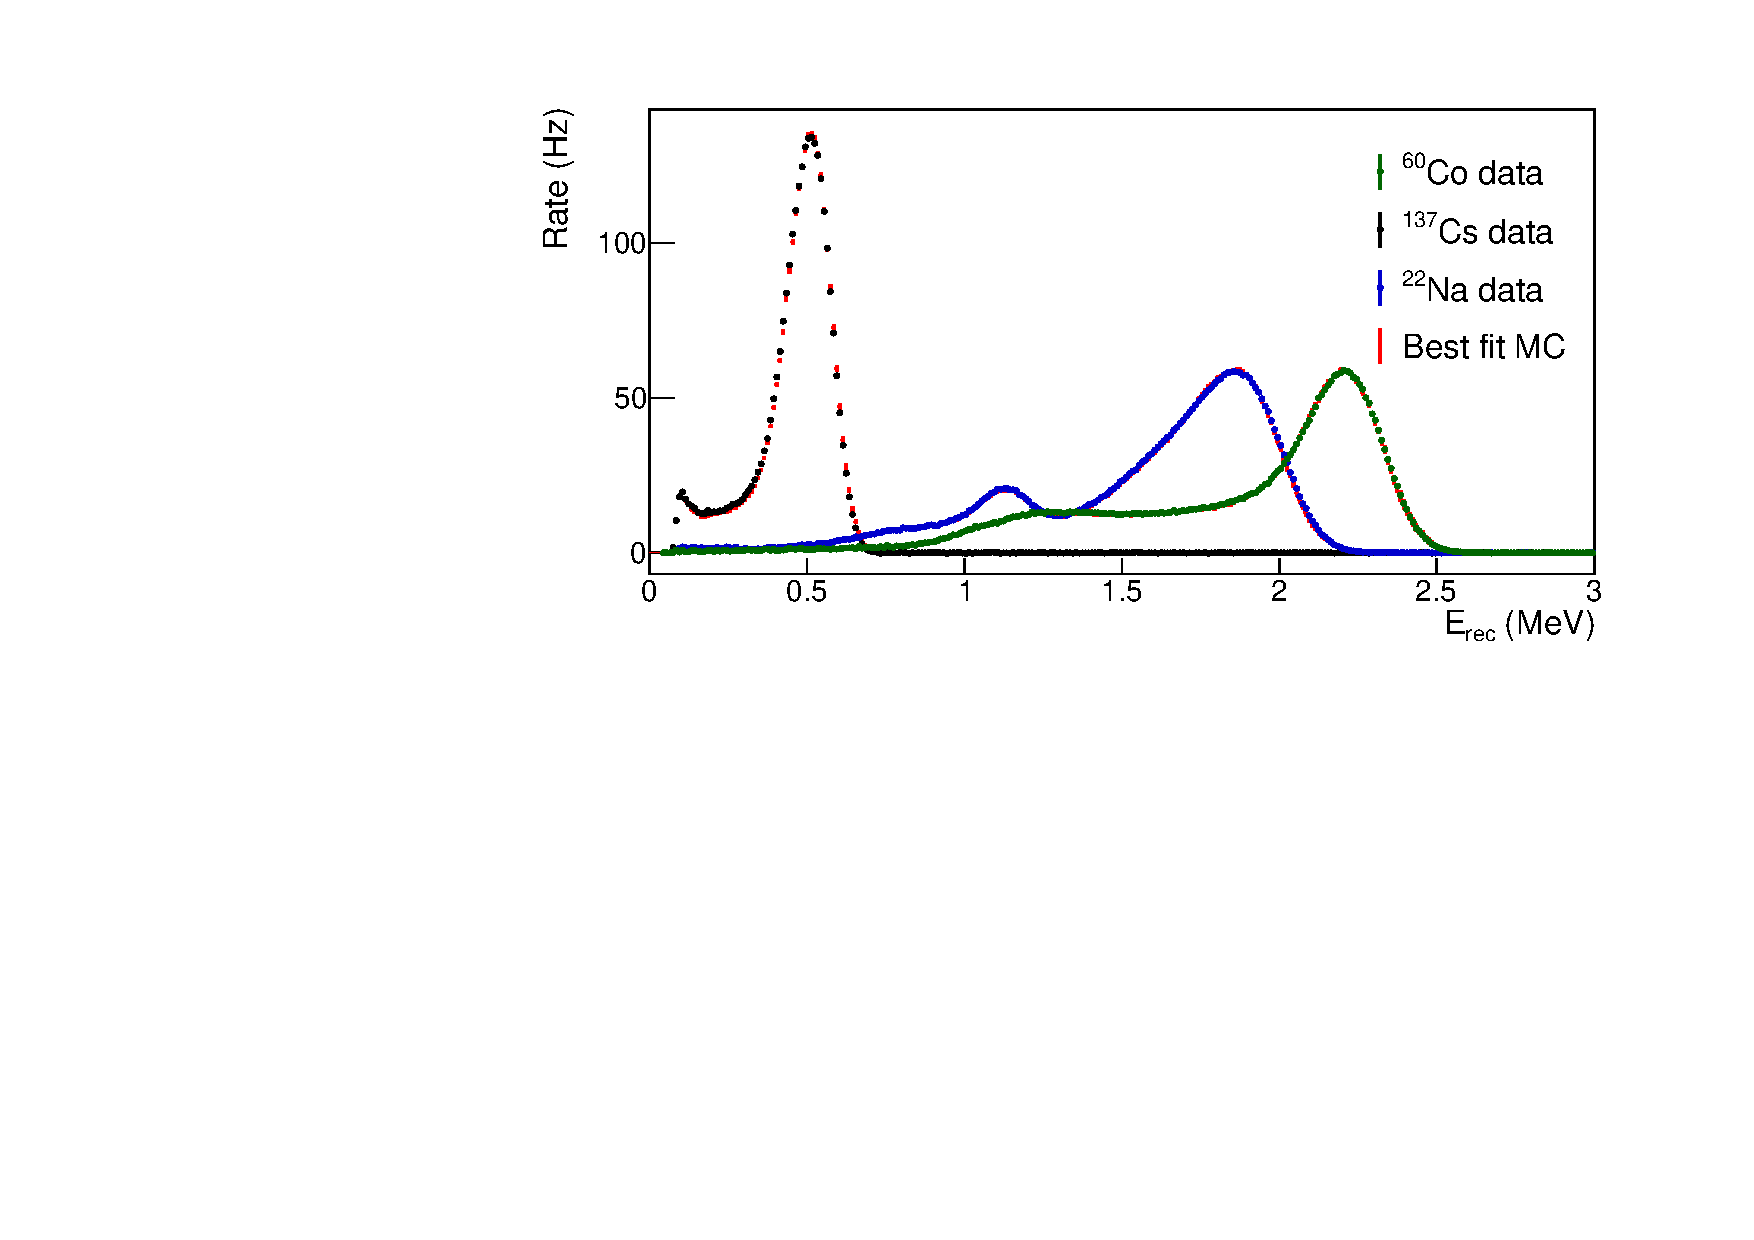
\includegraphics[width=0.45\textwidth]{CalibPaperPlot.pdf}
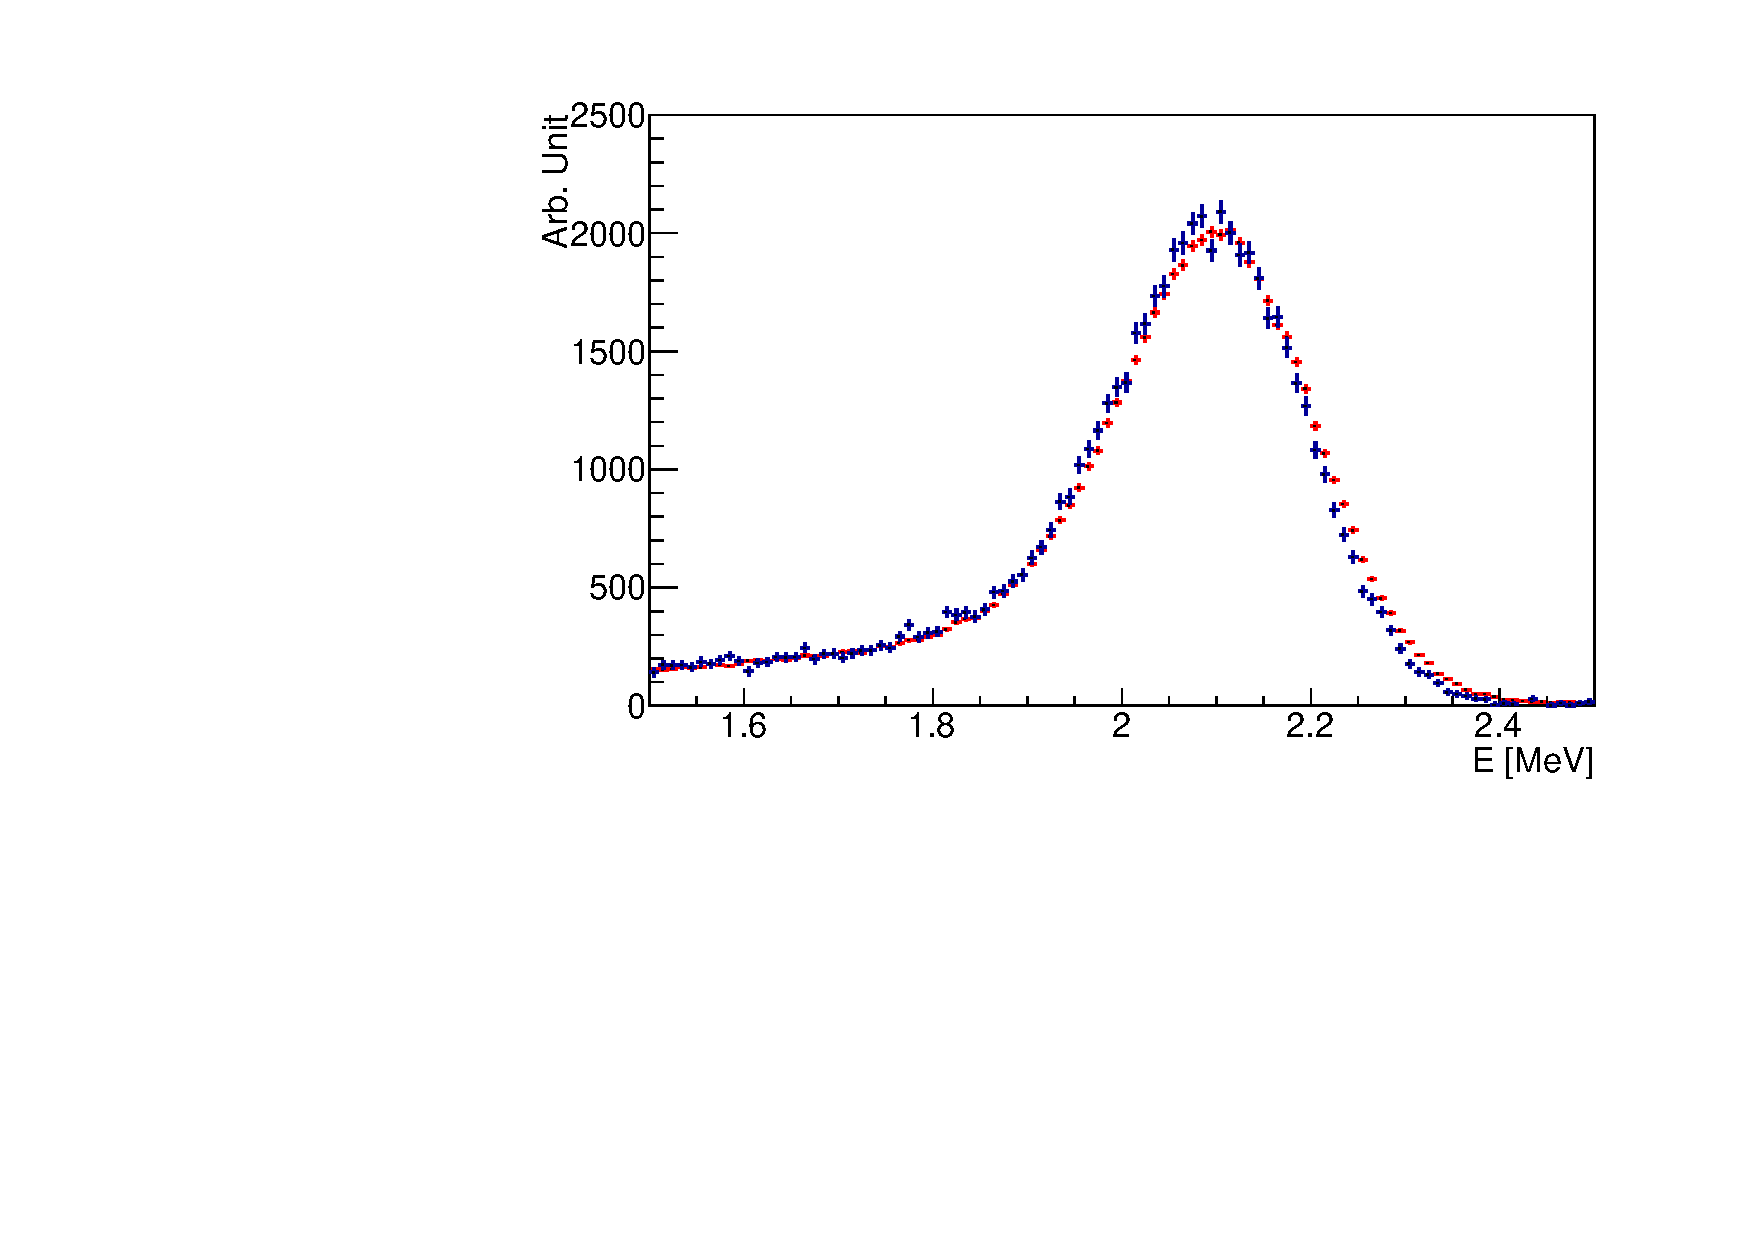
\includegraphics[width=0.45\textwidth]{hCf252v2.pdf}
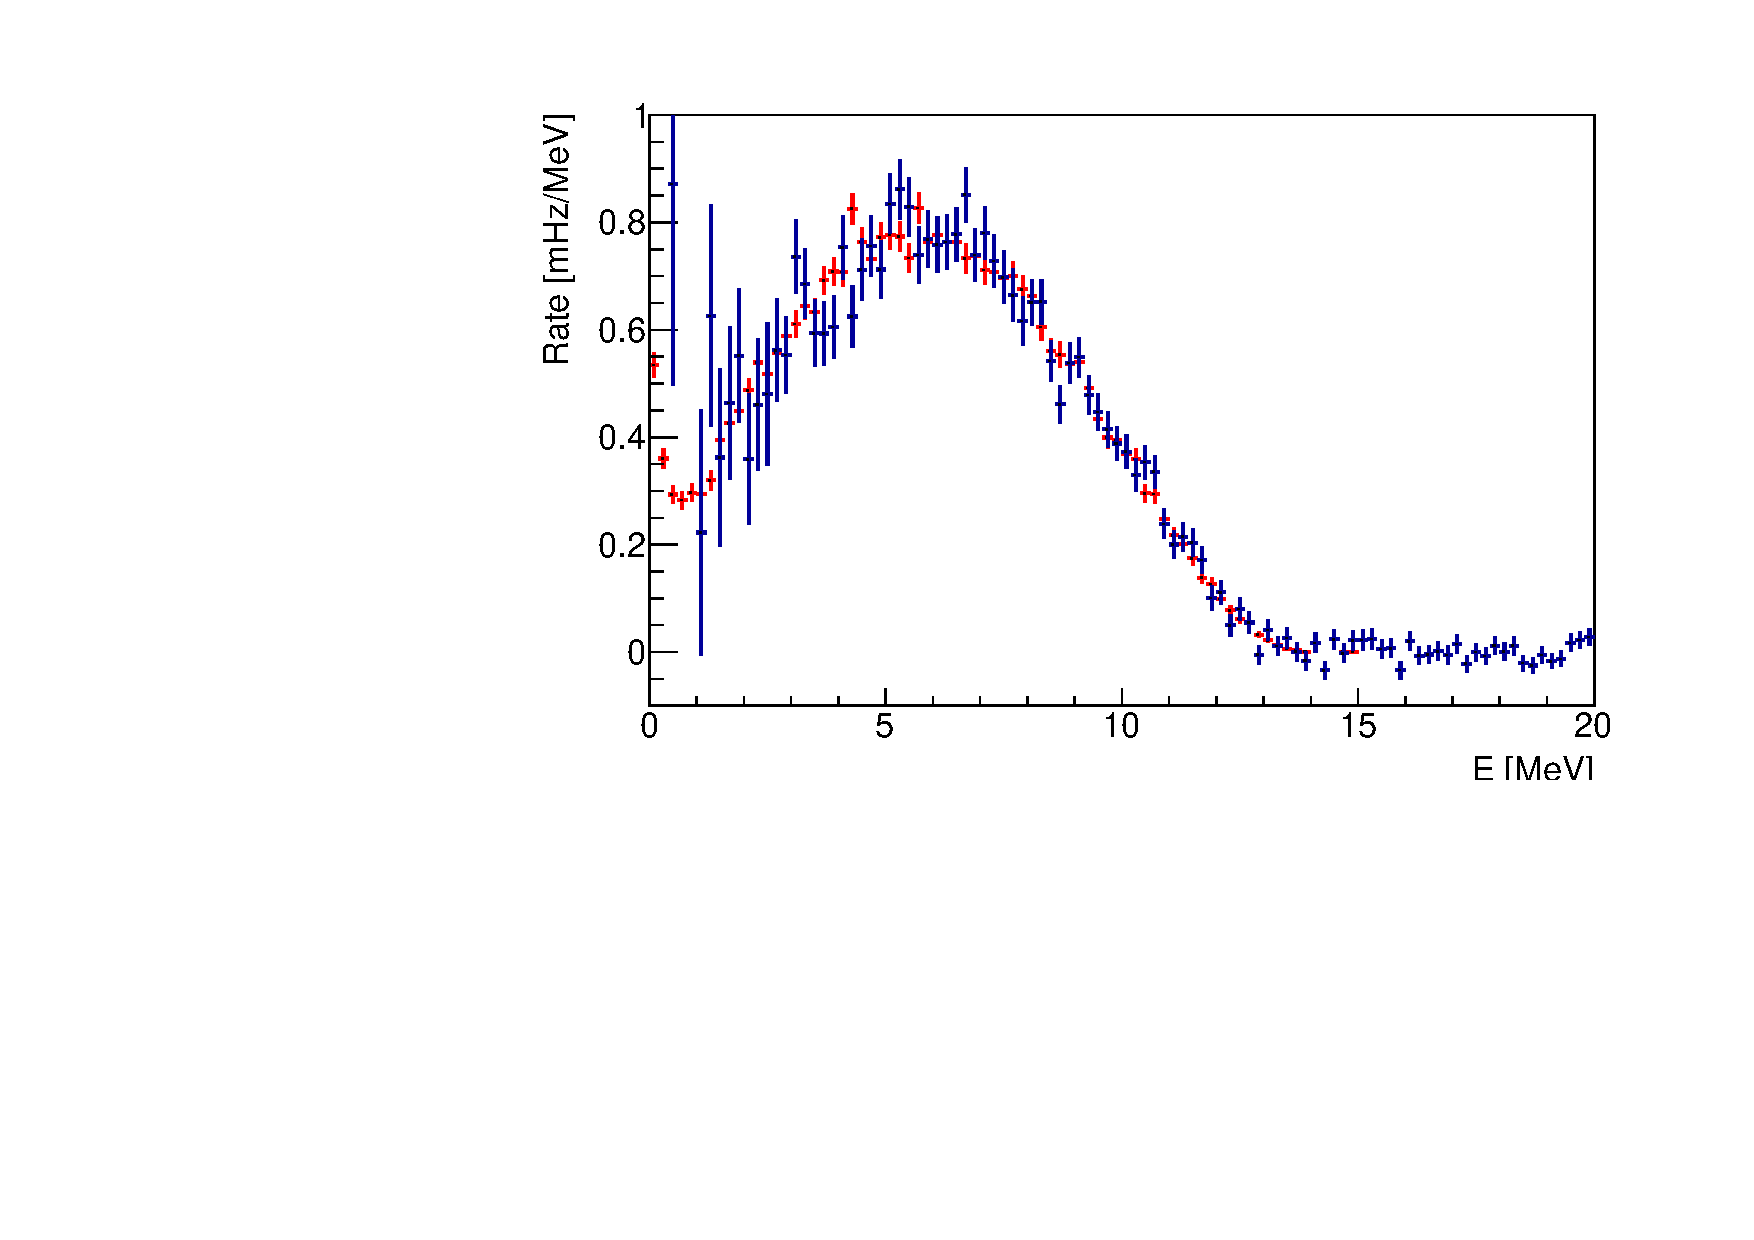
\includegraphics[width=0.45\textwidth]{hB12v2.pdf}
\caption{The calibration data compared with best fit MC spectrum. 
(Top left) Radioactive $\gamma$-ray source compared with best fit MC.
(Top right) Energy spectrum of $\gamma$-ray from neutron-hydrogen capture compared with best fit MC.
(Bottom) Energy spectrum of $^{12}$B $\beta$-decay compared with best fit MC.}
\label{fig:gammacalibration}
\end{figure}

\begin{figure}[h!]
\centering
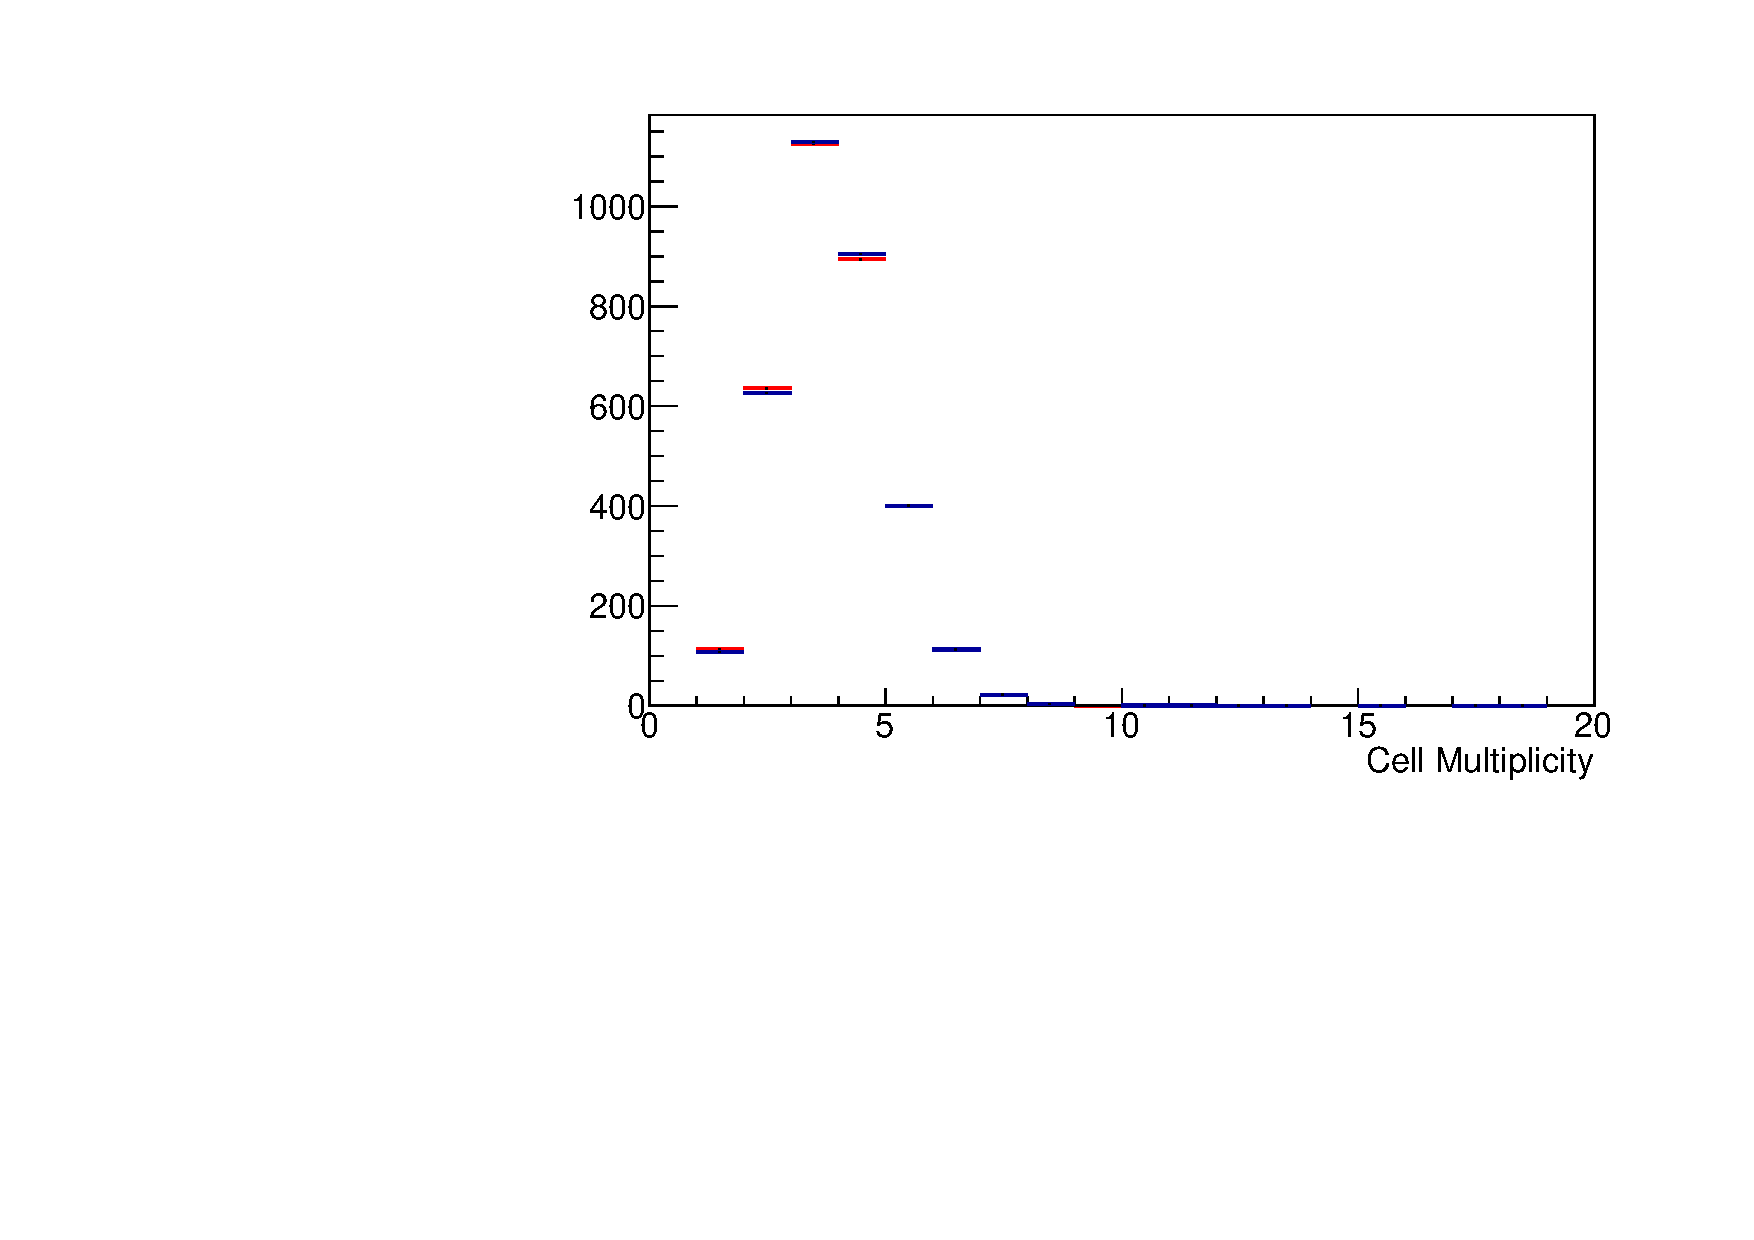
\includegraphics[width=0.45\textwidth]{hCo60multi.pdf}
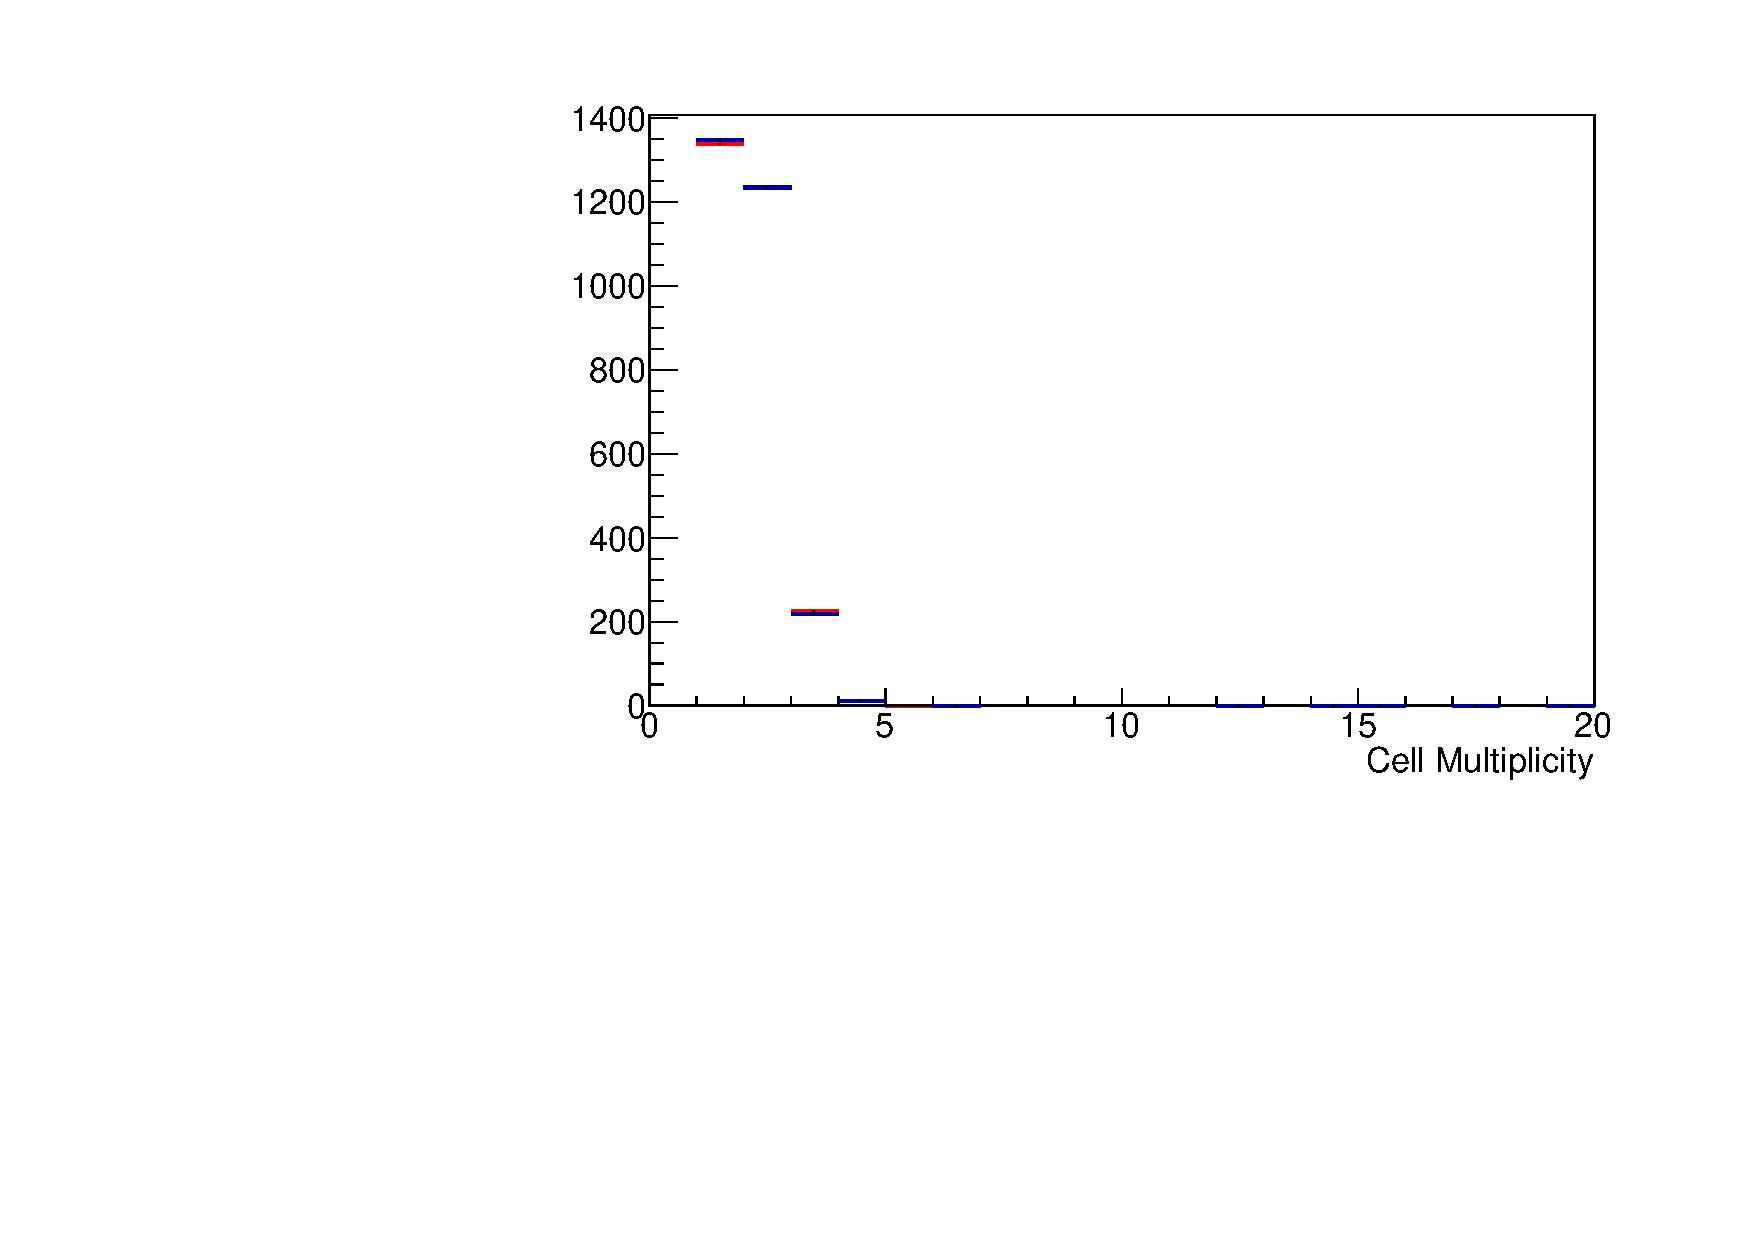
\includegraphics[width=0.45\textwidth]{hCs137multi.pdf}
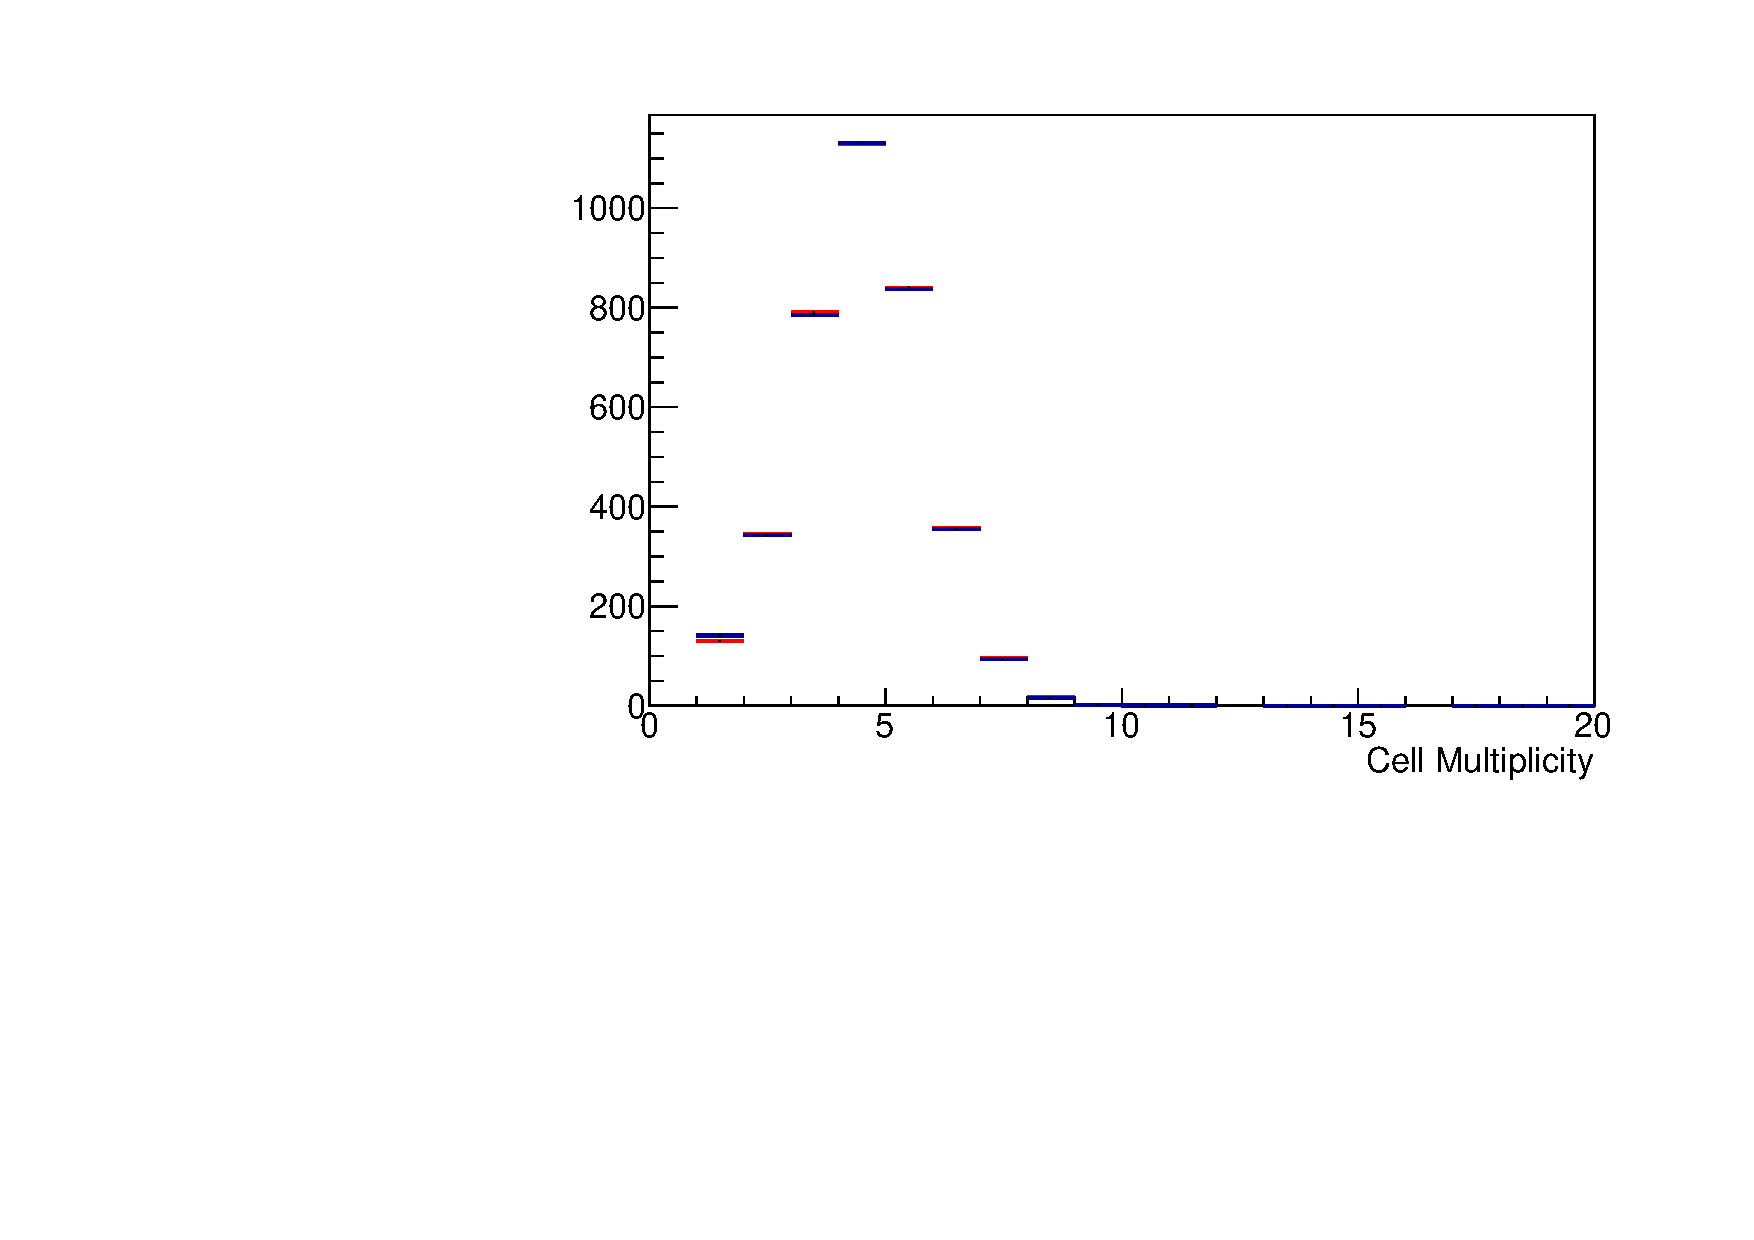
\includegraphics[width=0.45\textwidth]{hNa22mulit.pdf}
\caption{The multiplicity distribution of $\gamma$ calibration events. 
(Top left) Segment multiplicity of $^{60}$Co gamma events with data (MC) mean value $3.79\pm$BLAH ($3.85\pm$BLAH). 
(Top right) Segment multiplicity of $^{137}$Cs gamma events with data (MC) mean value $1.94\pm$BLAH ($1.94\pm$BLAH). 
(Bottom) Segment multiplicity of $^{22}$Na gamma events with data (MC) mean value $4.53\pm$BLAH ($4.50\pm$BLAH).}
\label{fig:multi}
\end{figure}

The scale of the reconstructed $\gamma$ energy is shown in Figure~\ref{fig:eresolution}, showing $<1\%$ difference between energy response model and reconstructed energy.
The end point of reconstructed (simulated) $\beta$ energy distribution was $13.36\pm0.18$~MeV ($13.15\pm0.08$~MeV), indicating good agreements between data-MC $\beta$ energy throughout the range of interest.
The segment multiplicity measured by gamma calibration also agreed well with MC within the systematic error from reconstructed energy scale.

\begin{figure}[h!]
\centering
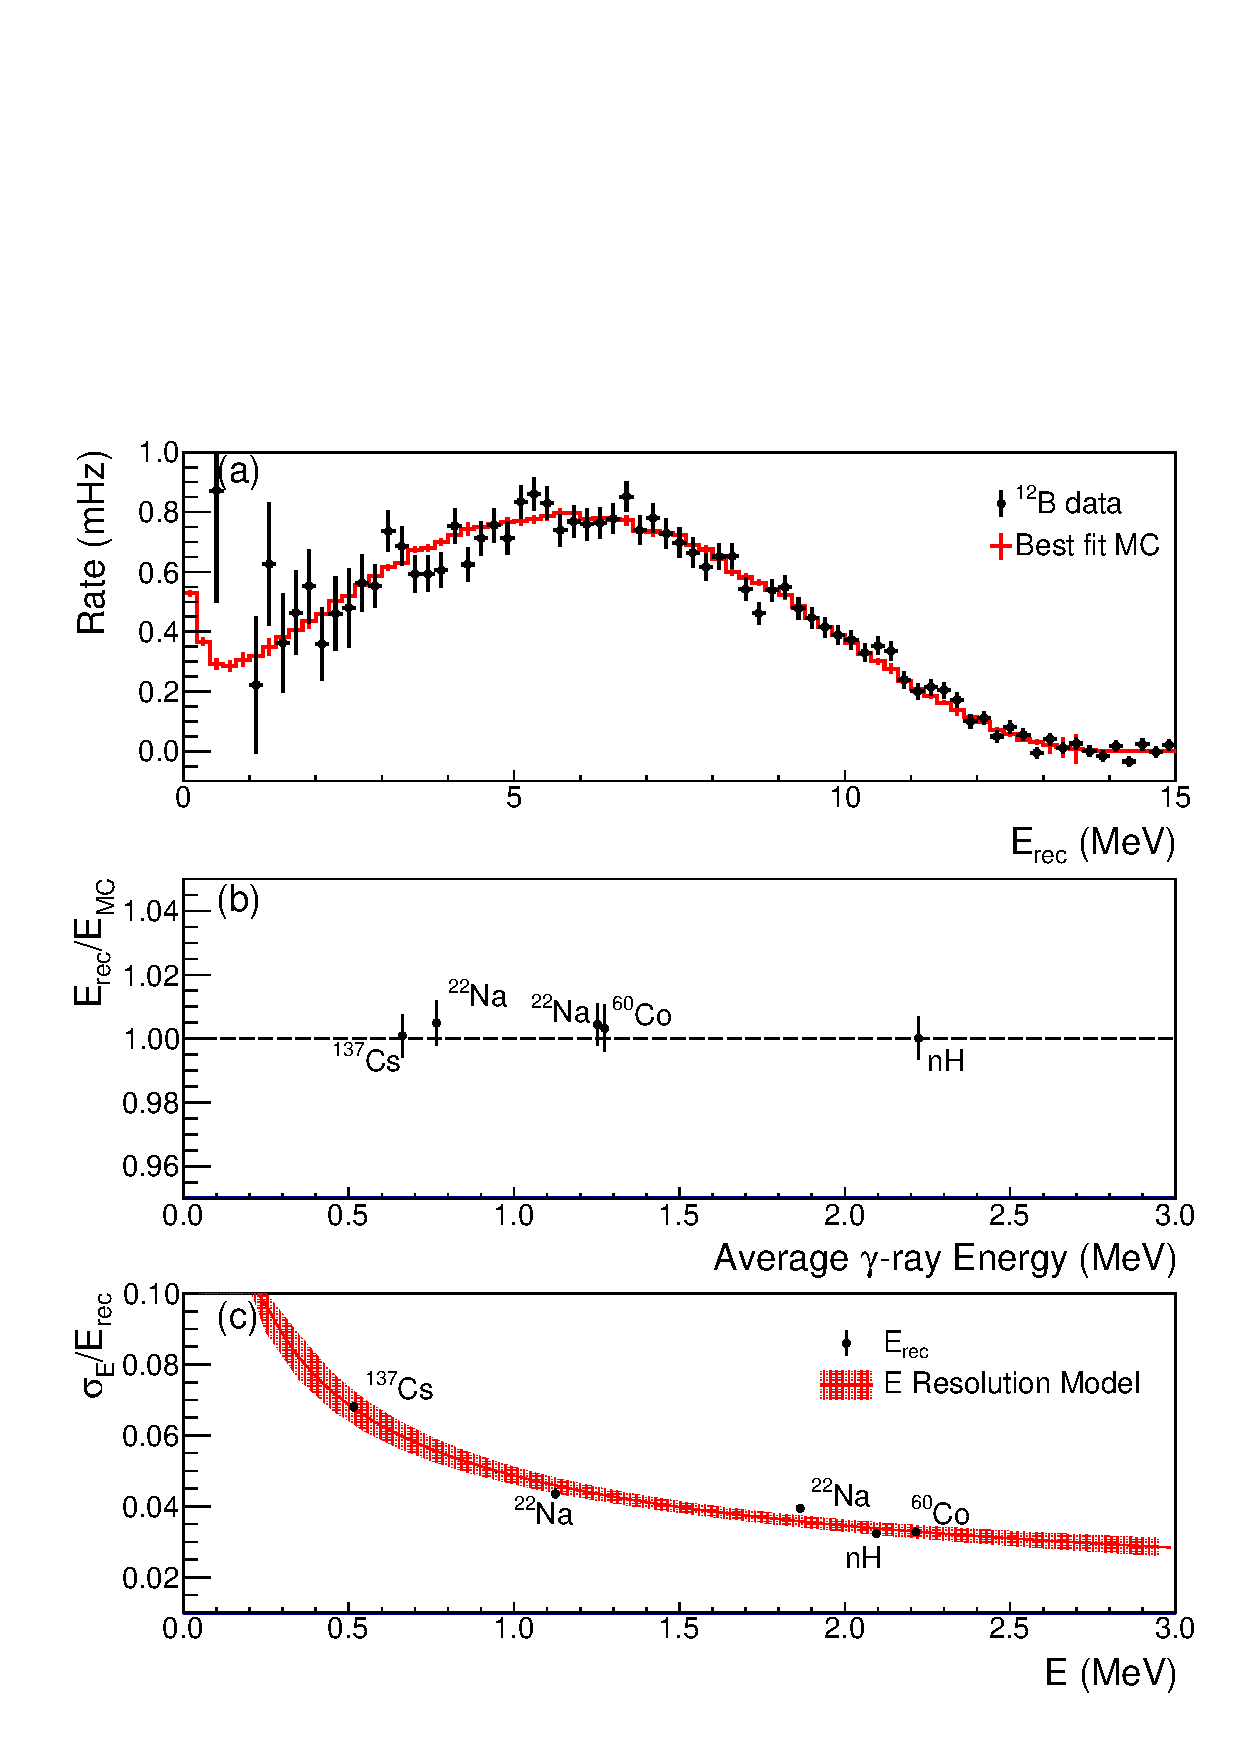
\includegraphics[trim = 0cm 0cm 0cm 7.2cm, clip,width=0.6\textwidth]{SpectPRLEScalePlot1.pdf}
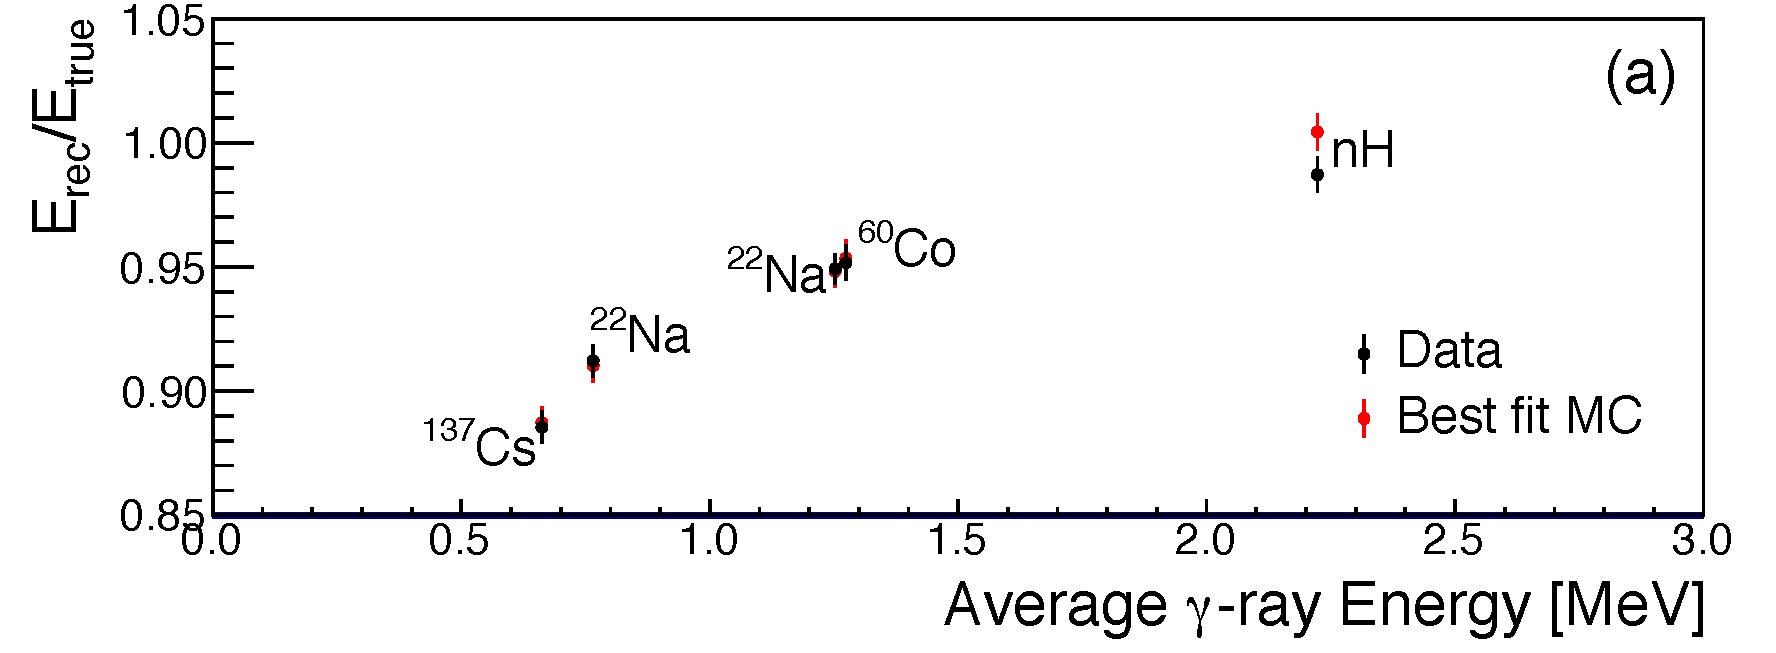
\includegraphics[width=0.6\textwidth]{nonlinear.pdf}
\caption{
(Top) The data-MC ratio of reconstructed $\gamma$ energy.
(Middle) The resolution of reconstructed energy.
(Bottom) Nonlinear reconstruction of $gamma$ energy}
\label{fig:eresolution}
\end{figure}

The resolution of reconstructed energy was also measured with the calibration $\gamma$-ray events, independent from the 5\% event-level energy resolution.
The best fit MC energy distributions were smeared with Gauss distribution individually until their $\chi^2$ from calibration data were minimized.
Each of the $\frac{\sigma_E}{E_{rec}}$ of the gauss smearing was plotted as the data points in Figure~\ref{fig:eresolution} bottom figure.
The resolution of all $\gamma$ energy calibration were fitted with a energy resolution function, 
\begin{equation}
    \frac{\sigma_E}{E_{rec}} = \sqrt{a^2+\frac{b^2}{E_{rec}}+\frac{c^2}{E^2_{rec}}},
\end{equation}
where $a$ is related to the light collection affected by detector geometry, $b$ is related to light yield of LS, and $c$ is related to quantum efficiency of PMTs.
The the best fit parameter of the function showed $\sim$4.8\% at 1 MeV.
With data-true energy ratio, the nonlinear reconstructed energy was also observed.

% E loss
The $^{22}$Na sources were deployed in various locations in the PROSPECT AD to characterize the $gamma$ energy loss because of limited detector active volume and the existence of the inactive volume. 
The sources are deployed at the corners, edges, and center of the detector.
The $\gamma$ energy spectra from source at different locations were compared with same MC setup.
As shown in Figure~\ref{fig:eloss}, the best fit MC energy spectra in one corner and the center of the detector successfully reproduced spectral feature caused by $\gamma$-ray escaped from detector.
The relative energy shifts between data and MC spectra was BLAH~keV. 

\begin{figure}[h!]
\centering
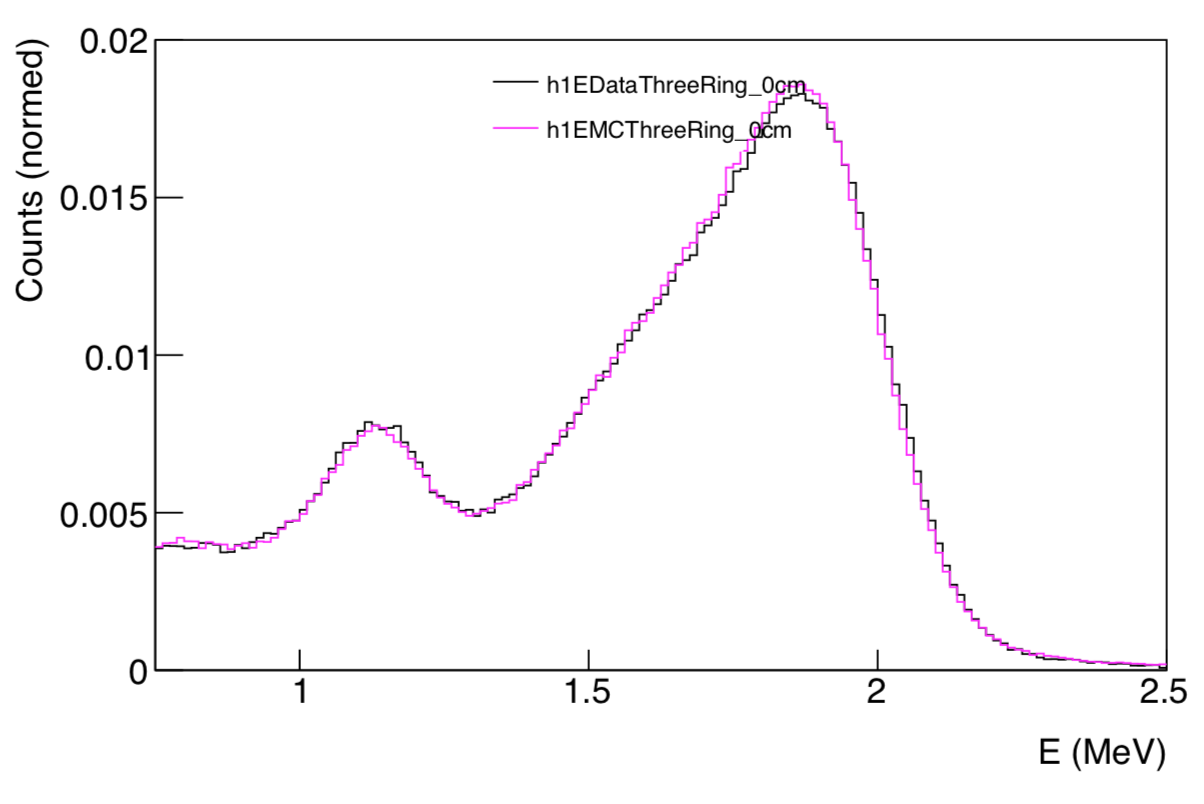
\includegraphics[width=0.45\textwidth]{elosscenter.png}
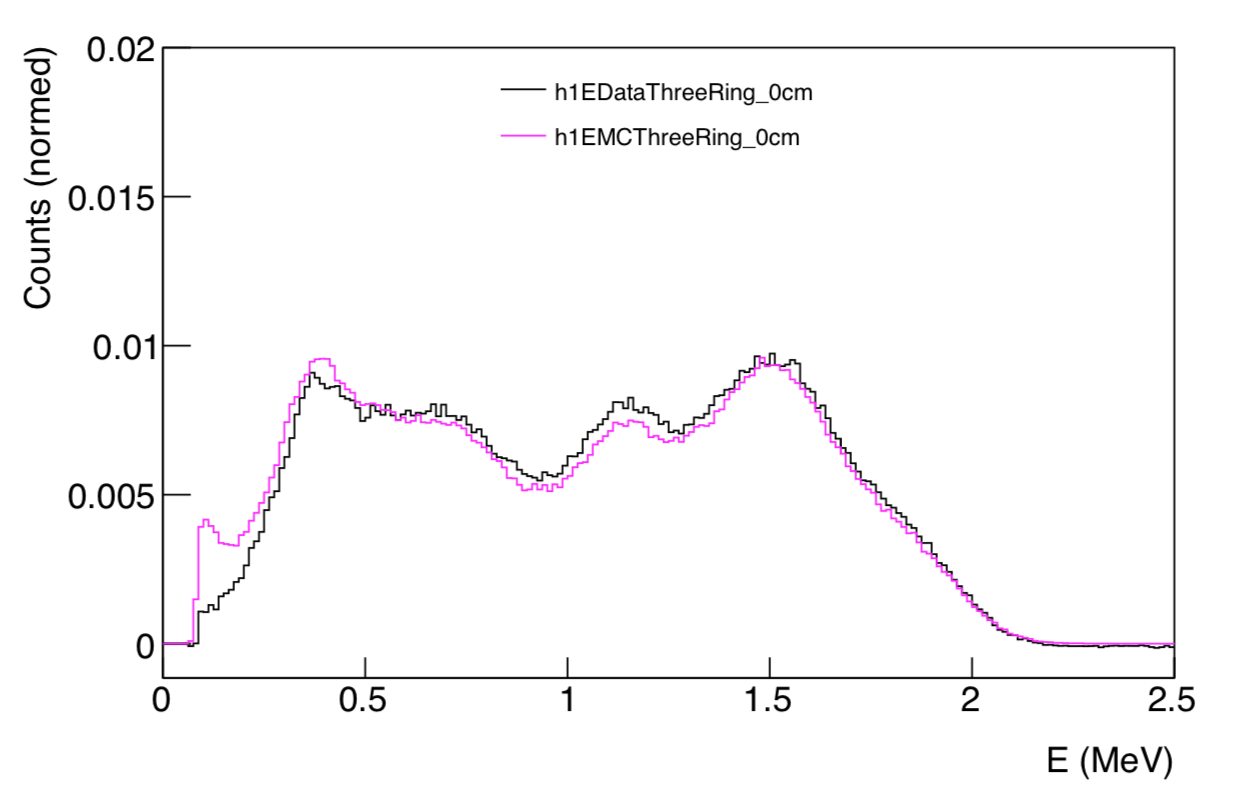
\includegraphics[width=0.45\textwidth]{elosscorner.png}
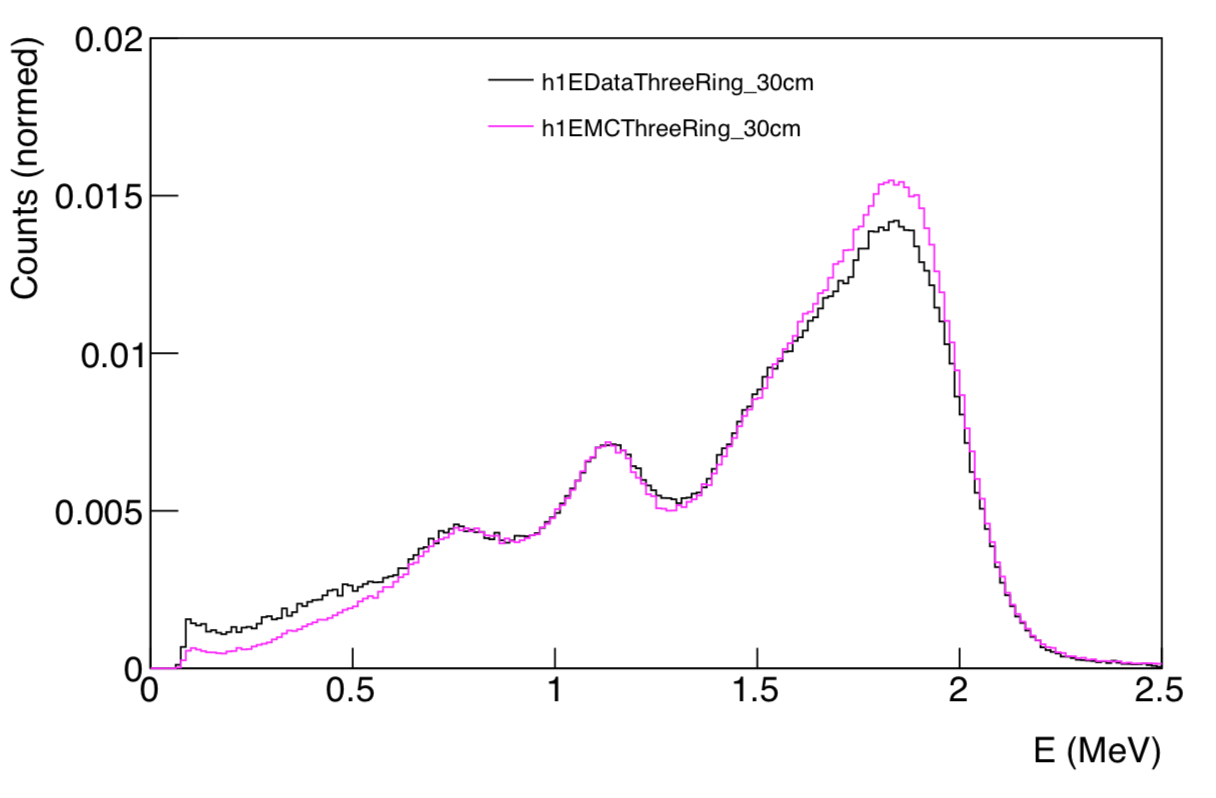
\includegraphics[width=0.45\textwidth]{eloss30.png}
\caption{
(Top left) The $gamma$ energy of $^{22}$Na source at the center of AD compared with best fit MC.
(Top right) The $gamma$ energy of $^{22}$Na source at one corner of AD compared with best fit MC.
(Bottom) The $gamma$ energy of $^{22}$Na source at center of AD, but 30~cm closer to one PMT, compared with best fit MC.}
\label{fig:eloss}
\end{figure}

% Cross-calibration check
% Cross-detector check
The best fit response model was found from first one of the three energy scale calibrations during the data acquisition period.
The calibration sources were also deployed in different locations.
Additional calibration simulations were also organized to compare with later two calibrations.
The cross-calibration comparison is shown in Figure~\ref{fig:compare}. 
The data-MC ratio of each $\gamma$ source calibration differed within the $1\%$ energy scale uncertainty.
As the $^{137}$Cs and $^{22}$Na sources were deployed in various locations in the detector the data-MC ratio of energy scale was also made throughout the detector geometry.
The energy scale of at different locations of detector varies within $BLAH\%$, as shown in Figure~\ref{fig:compare}.

\begin{figure}[h!]
\centering
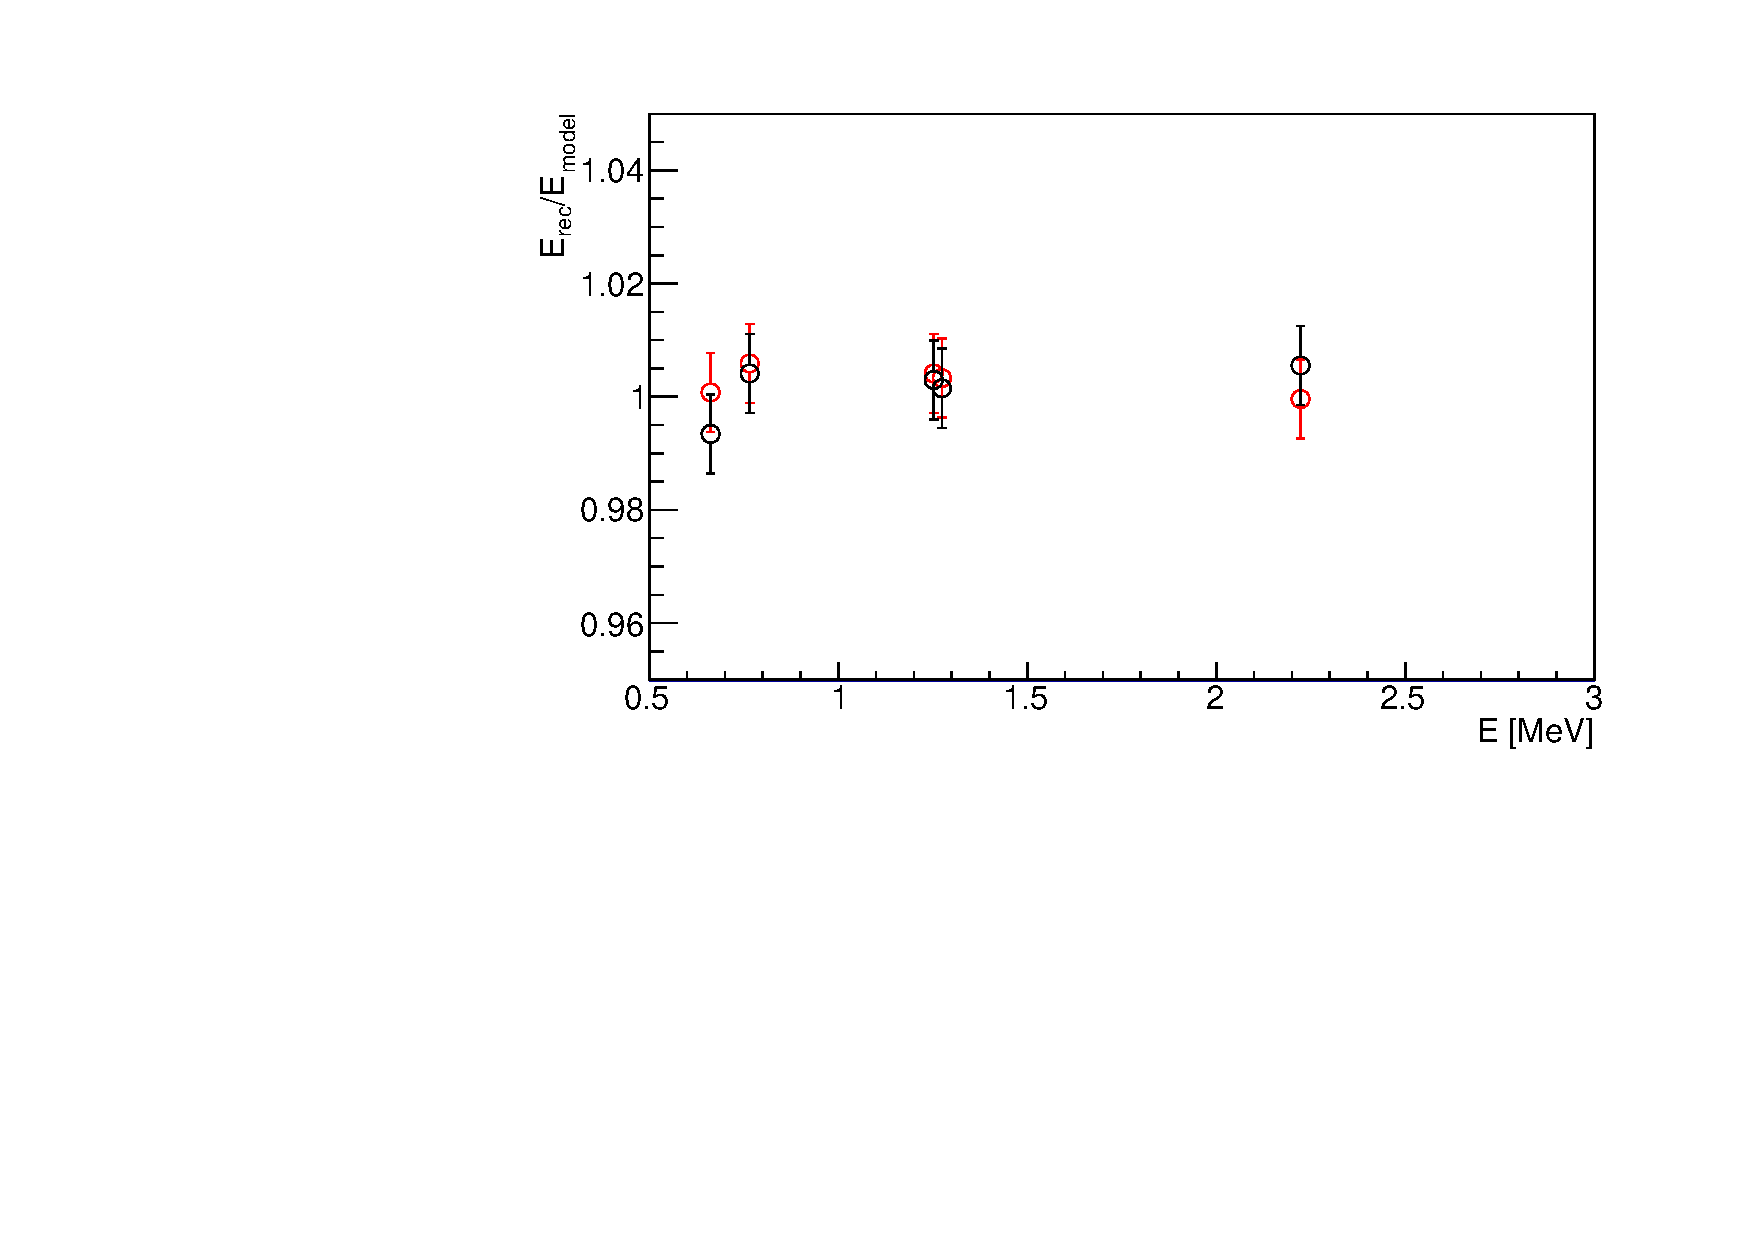
\includegraphics[width=0.6\textwidth]{EScaleCompare.pdf}
\includegraphics[width=0.6\textwidth, height=0.1\textheight]{data-MC_scale_in_different_positions.pdf}
\caption{
(Top) The comparison of data-MC scale among the two (TODO: three) calibrations.
(Bottom) The data-MC scale at different positions in the detector.
}
\label{fig:compare}
\end{figure}

The detector response matrices were generated individually for neutrino oscillation and energy spectrum analysis.
The response matrix for oscillation analysis was, shown in Figure~\ref{matrix}. (TODO: bin description, L:E).
The response matrix for oscillation was shown in Figure~\ref{matrix}. (TODO: bin description, E only).

\begin{figure}[h!]
\centering
\includegraphics[width=0.45\textwidth]{LvsE_Response_Matrix.pdf}
\includegraphics[width=0.45\textwidth]{E_Response_Matrix.pdf}
\caption{
(Left) Baseline dependent detector response matrix for oscillation analysis.
(Right) The detector response matrix for spectrum analysis.
}
\label{fig:matrix}
\end{figure}

\section{TODO LIST}
\begin{itemize}
    \item Rerun data analysis for 2018c release. This is vital to update the 5\% resolution smearing and 85~keV analysis threshold since LS has changed.
    \item Calibration analysis for 2018 Dec. calibration campaign. Check if the best fit E response model works on latest calibration. Strengthen the E scale study with AmBe and BiPo.
    \item Then every plots should be remade.
    \item Clean language.
\end{itemize}

\end{document}
